In this section we report the results of $\WW$ cross-section measurements in 
different jet bin or final states. The measurements are performed in the 
dataset corresponding to an integrated luminosity of  $\intlumiEightTeV$.
The data driven background estimates are evaluated consistently for each jet bin.

\subsection{Measurements in the 0-Jet bin}

Table~\ref{tab:datayields_wwxsec_0j} shows the expected number of signal and background events,
as well as the signal acceptance and measured cross section in each lepton channel.
Table ~\ref{tab:datayields_wwxsec_0j_incl} shows the results including all lepton channels.
The kinematic distributions of the events selected are shown in Figures \ref{fig:xs_kinematics_mm_0j} - \ref{fig:xs_kinematics_incl_0j}.

\begin{table}[!ht]
{\small
\begin{center}
\begin{tabular}{|l|c|c|c|c|}
\hline
Sample  & mm    & me    & em    & ee    \\ \hline
$qqWW$  & $139.43 \pm 2.28 \pm 10.09 $  & $188.02 \pm 2.63 \pm 13.25 $  & $227.65 \pm 2.95 \pm 16.04 $  & $89.98 \pm 1.85 \pm 6.94 $    \\
$qqWW$  & $10.00 \pm 0.45 \pm 3.08 $    & $11.74 \pm 0.48 \pm 3.60 $    & $14.77 \pm 0.57 \pm 4.53 $    & $7.03 \pm 0.39 \pm 2.17 $ \\
$t\bar{t} + tW$ & $27.05 \pm 3.15 \pm 5.84 $    & $36.70 \pm 3.73 \pm 7.93 $    & $47.65 \pm 4.22 \pm 10.29 $   & $19.49 \pm 2.81 \pm 4.21 $    \\
$W+jets$    & $9.87 \pm 3.02 \pm 3.55 $ & $10.97 \pm 2.19 \pm 3.95 $    & $26.67 \pm 3.33 \pm 9.60 $    & $8.76 \pm 1.03 \pm 3.15 $ \\
$WZ$    & $5.54 \pm 0.19 \pm 0.63 $ & $4.51 \pm 0.18 \pm 0.50 $ & $6.99 \pm 0.21 \pm 0.78 $ & $3.05 \pm 0.14 \pm 0.35 $ \\
$ZZ$    & $4.47 \pm 0.14 \pm 0.44 $ & $0.18 \pm 0.02 \pm 0.02 $ & $0.26 \pm 0.02 \pm 0.03 $ & $2.93 \pm 0.12 \pm 0.30 $ \\
$Z/\gamma*$ & $24.78 \pm 5.19 \pm 6.06 $    & $0.11 \pm 0.11 \pm 0.01 $ & $0.69 \pm 0.29 \pm 0.07 $ & $15.53 \pm 4.93 \pm 3.80 $    \\
$W\gamma*/W+\gamma$ & $0.37 \pm 0.14 \pm 0.11 $ & $2.61 \pm 1.08 \pm 0.78 $ & $4.65 \pm 1.27 \pm 1.40 $ & $13.06 \pm 2.91 \pm 3.92 $    \\
\hline \hline
Total B.    & $72.07 \pm 6.79 \pm 9.17 $    & $55.08 \pm 6.45 \pm 7.59 $    & $86.92 \pm 5.54 \pm 14.17 $   & $62.82 \pm 6.45 \pm 7.59 $    \\ \hline \hline
Total B.+S. & $221.50 \pm 7.17 \pm 13.98 $  & $254.84 \pm 6.99 \pm 15.69 $  & $329.34 \pm 6.30 \pm 21.88 $  & $159.83 \pm 6.72 \pm 10.51 $  \\ \hline \hline
Data    & $241$     & $308$     & $396$     & $158$     \\ \hline \hline
Acceptance ( \% )   & $0.70 \pm 0.06    $& $0.94 \pm 0.07   $& $1.14 \pm 0.09   $& $0.46 \pm 0.04   $\\
Cross Section ( pb )    & $64.56 \pm 5.93 \pm 6.73$     & $72.31 \pm 5.02 \pm 6.29$     & $72.81 \pm 4.69 \pm 6.69$     & $56.03 \pm 7.40 \pm 7.52$     \\ \hline
\end{tabular}
\caption{Summary of yields for 0-jet channel.Uncertainties on yields and cross sections are $\mathrm{(stat.)} \pm \mathrm{(syst.)}$. The systematic uncertainty on the cross section does not include the luminosity}
\label{tab:datayields_wwxsec_0j}
\end{center}}
\end{table}

\begin{table}[!ht]
{\small
\begin{center}
\begin{tabular}{|l|c|c|c|c|}
\hline
Sample  & incl  \\ \hline
$qqWW$  & $645.07 \pm 4.92 \pm 46.33 $  \\
$qqWW$  & $43.54 \pm 0.96 \pm 13.38 $   \\
$t\bar{t} + tW$ & $130.89 \pm 7.04 \pm 28.27 $  \\
$W+jets$    & $56.27 \pm 5.11 \pm 20.26 $   \\
$WZ$    & $20.09 \pm 0.36 \pm 2.27 $    \\
$ZZ$    & $7.84 \pm 0.19 \pm 0.78 $ \\
$Z/\gamma*$ & $41.11 \pm 7.16 \pm 9.86 $    \\
$W\gamma*/W+\gamma$ & $20.70 \pm 3.35 \pm 6.21 $    \\
\hline \hline
Total B.    & $276.90 \pm 11.76 \pm 36.76 $ \\ \hline \hline
Total B.+S. & $965.51 \pm 12.78 \pm 60.63 $ \\ \hline \hline
Data    & $1103$    \\ \hline \hline
Acceptance ( \% )   & $3.23 \pm 0.26    $\\
Cross Section ( pb )    & $68.51 \pm 2.75 \pm 6.28$     \\ \hline
\end{tabular}
\caption{Summary of yields for 0-jet channel.Uncertainties on yields and cross sections are $\mathrm{(stat.)} \pm \mathrm{(syst.)}$. The systematic uncertainty on the cross section does not include the luminosity}
\label{tab:datayields_wwxsec_0j_incl}
\end{center}}
\end{table}

\begin{figure}[!hbtp]
\centering
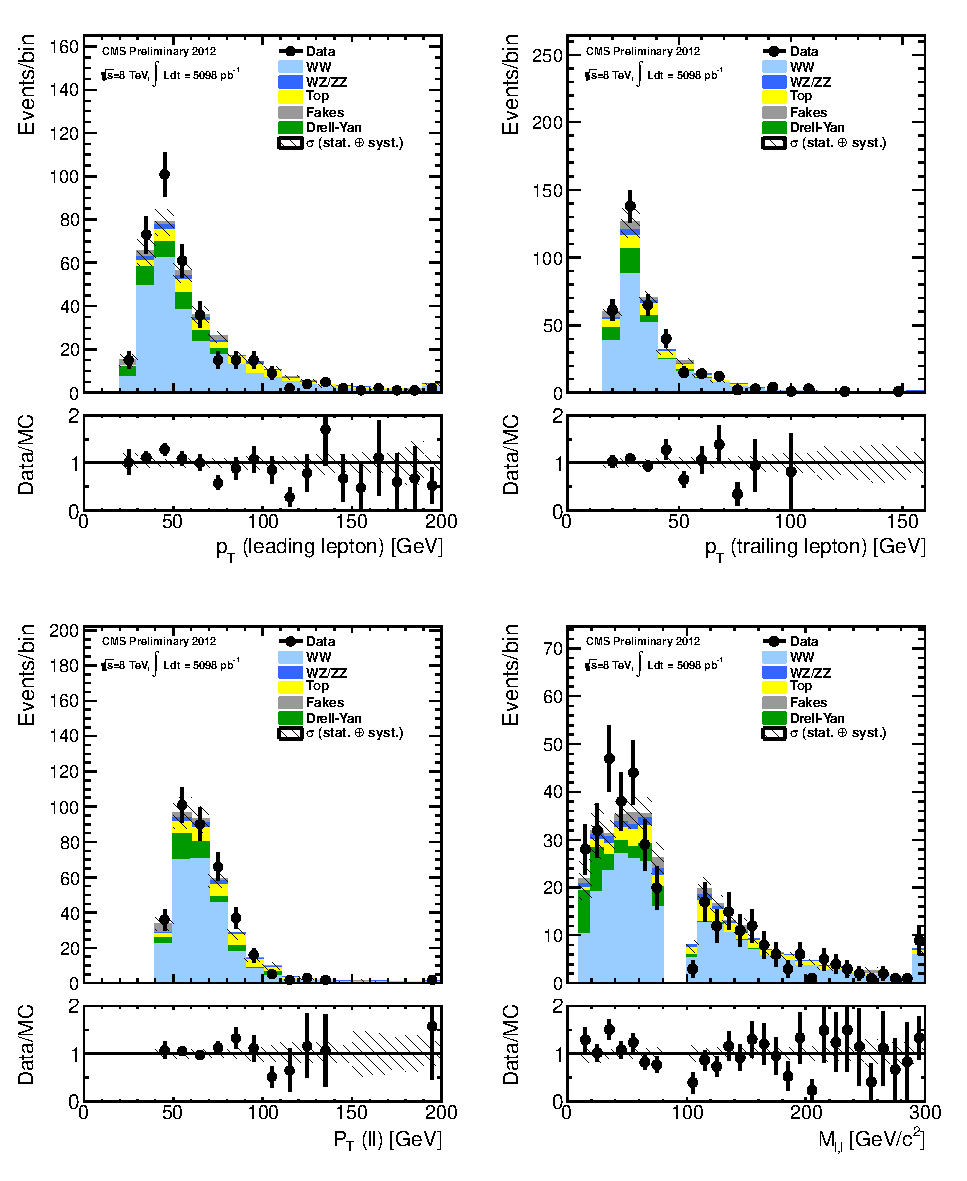
\includegraphics[width=1\textwidth]{figures/ww_analysis20_0_ALL_mm_0j.pdf}
\caption{Kinematic distributions in the $\mu\mu$ final state in the 0-jet bin.}
\label{fig:xs_kinematics_mm_0j}
\end{figure}
\begin{figure}[!hbtp]
\centering
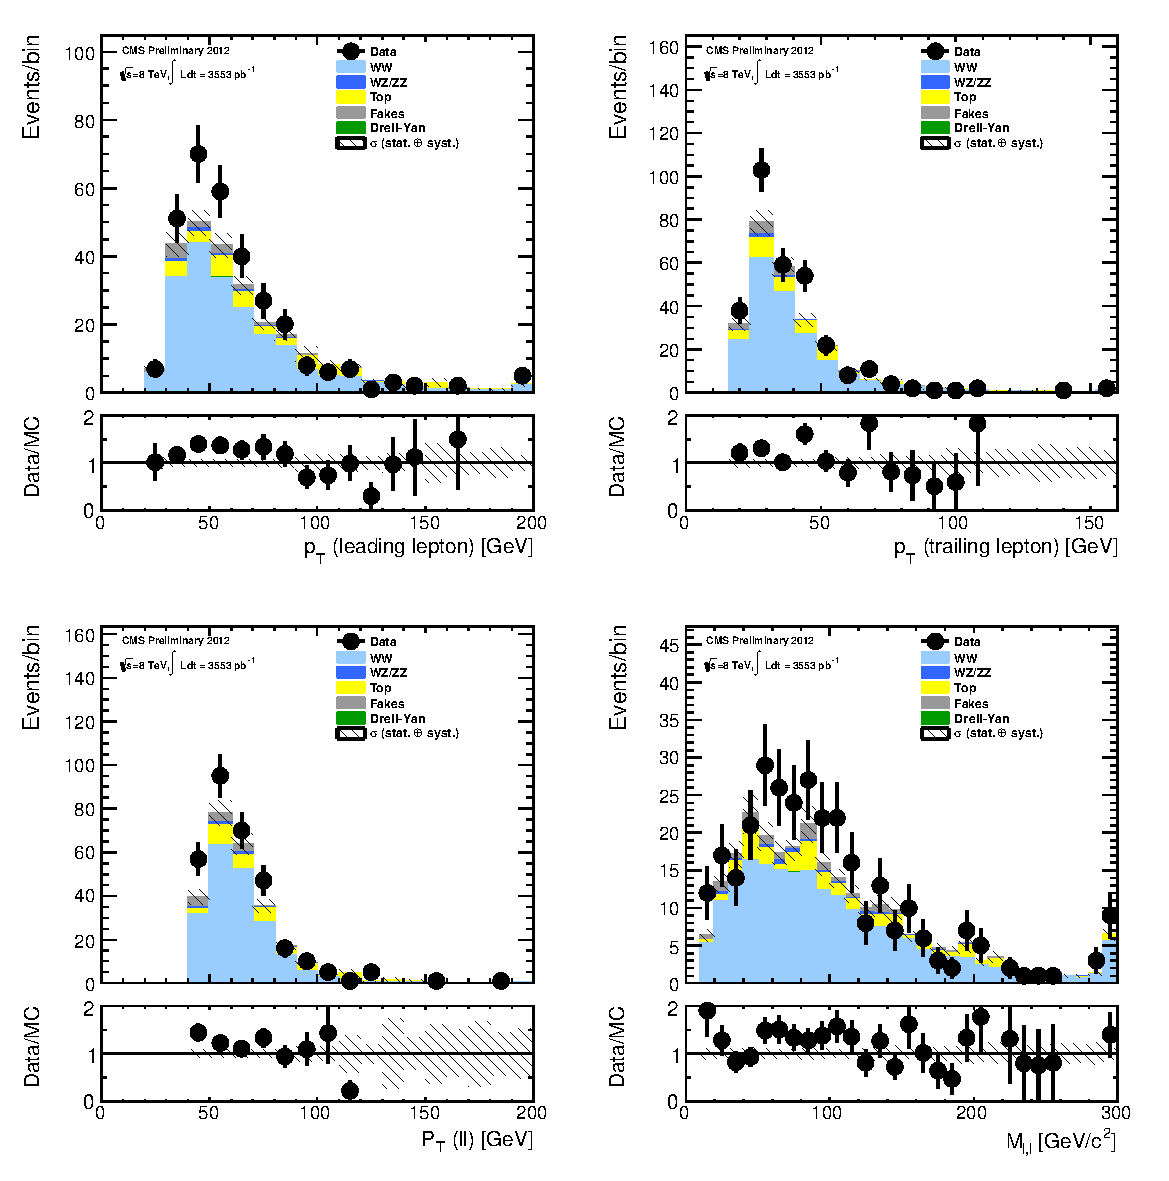
\includegraphics[width=1\textwidth]{figures/ww_analysis20_0_ALL_me_0j.pdf}
\caption{Kinematic distributions in the $\mu e$ final state in the 0-jet bin.}
\label{fig:xs_kinematics_me_0j}
\end{figure}
\begin{figure}[!hbtp]
\centering
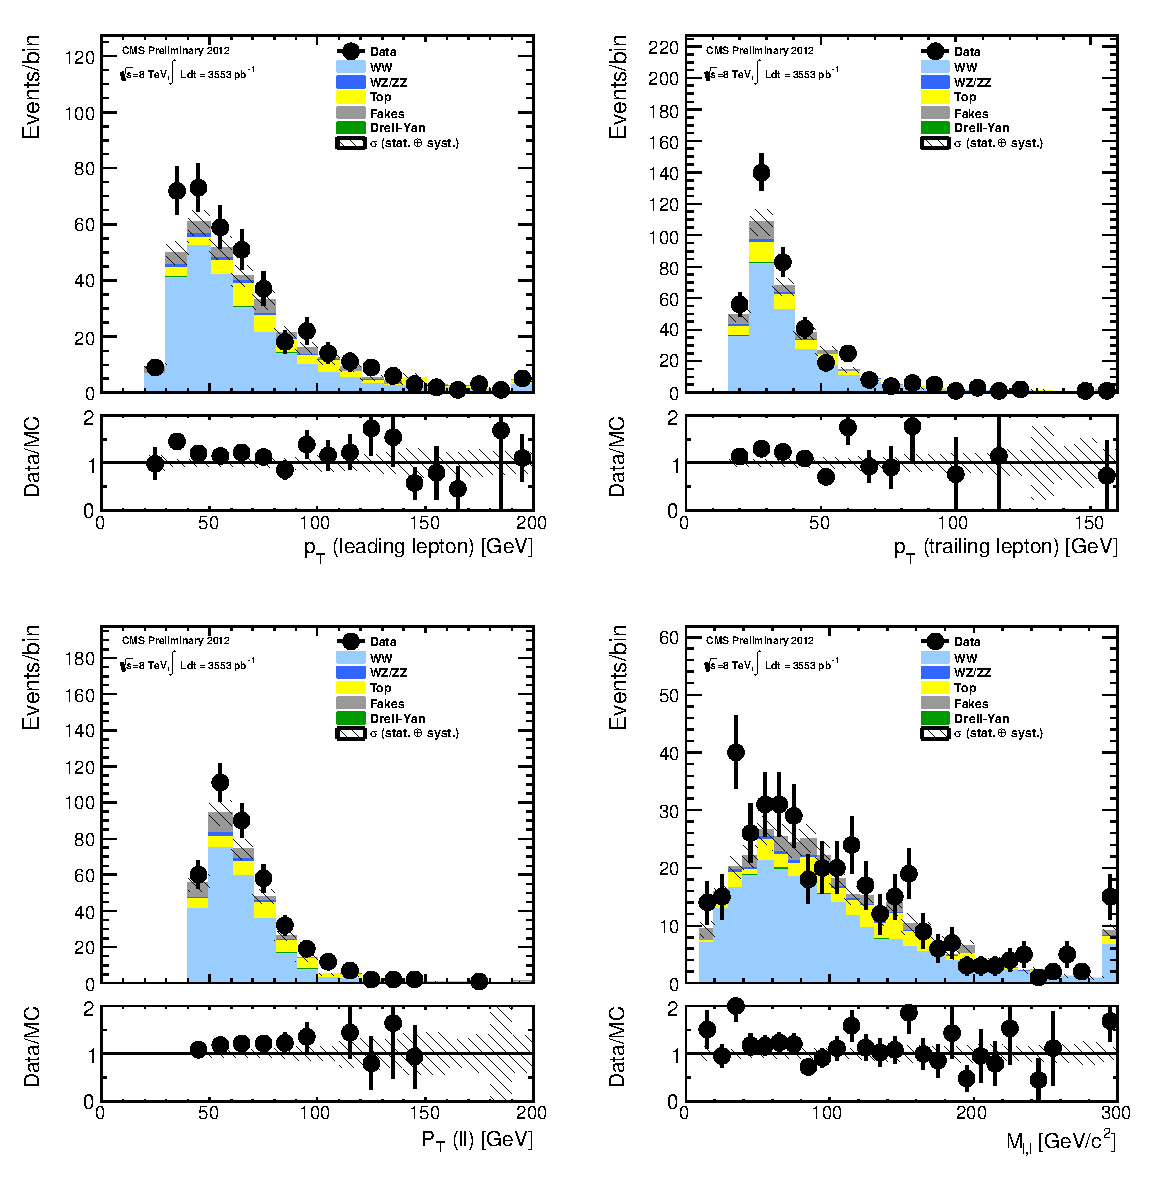
\includegraphics[width=1\textwidth]{figures/ww_analysis20_0_ALL_em_0j.pdf}
\caption{Kinematic distributions in the $e\mu$ final state in the 0-jet bin.}
\label{fig:xs_kinematics_em_0j}
\end{figure}
\begin{figure}[!hbtp]
\centering
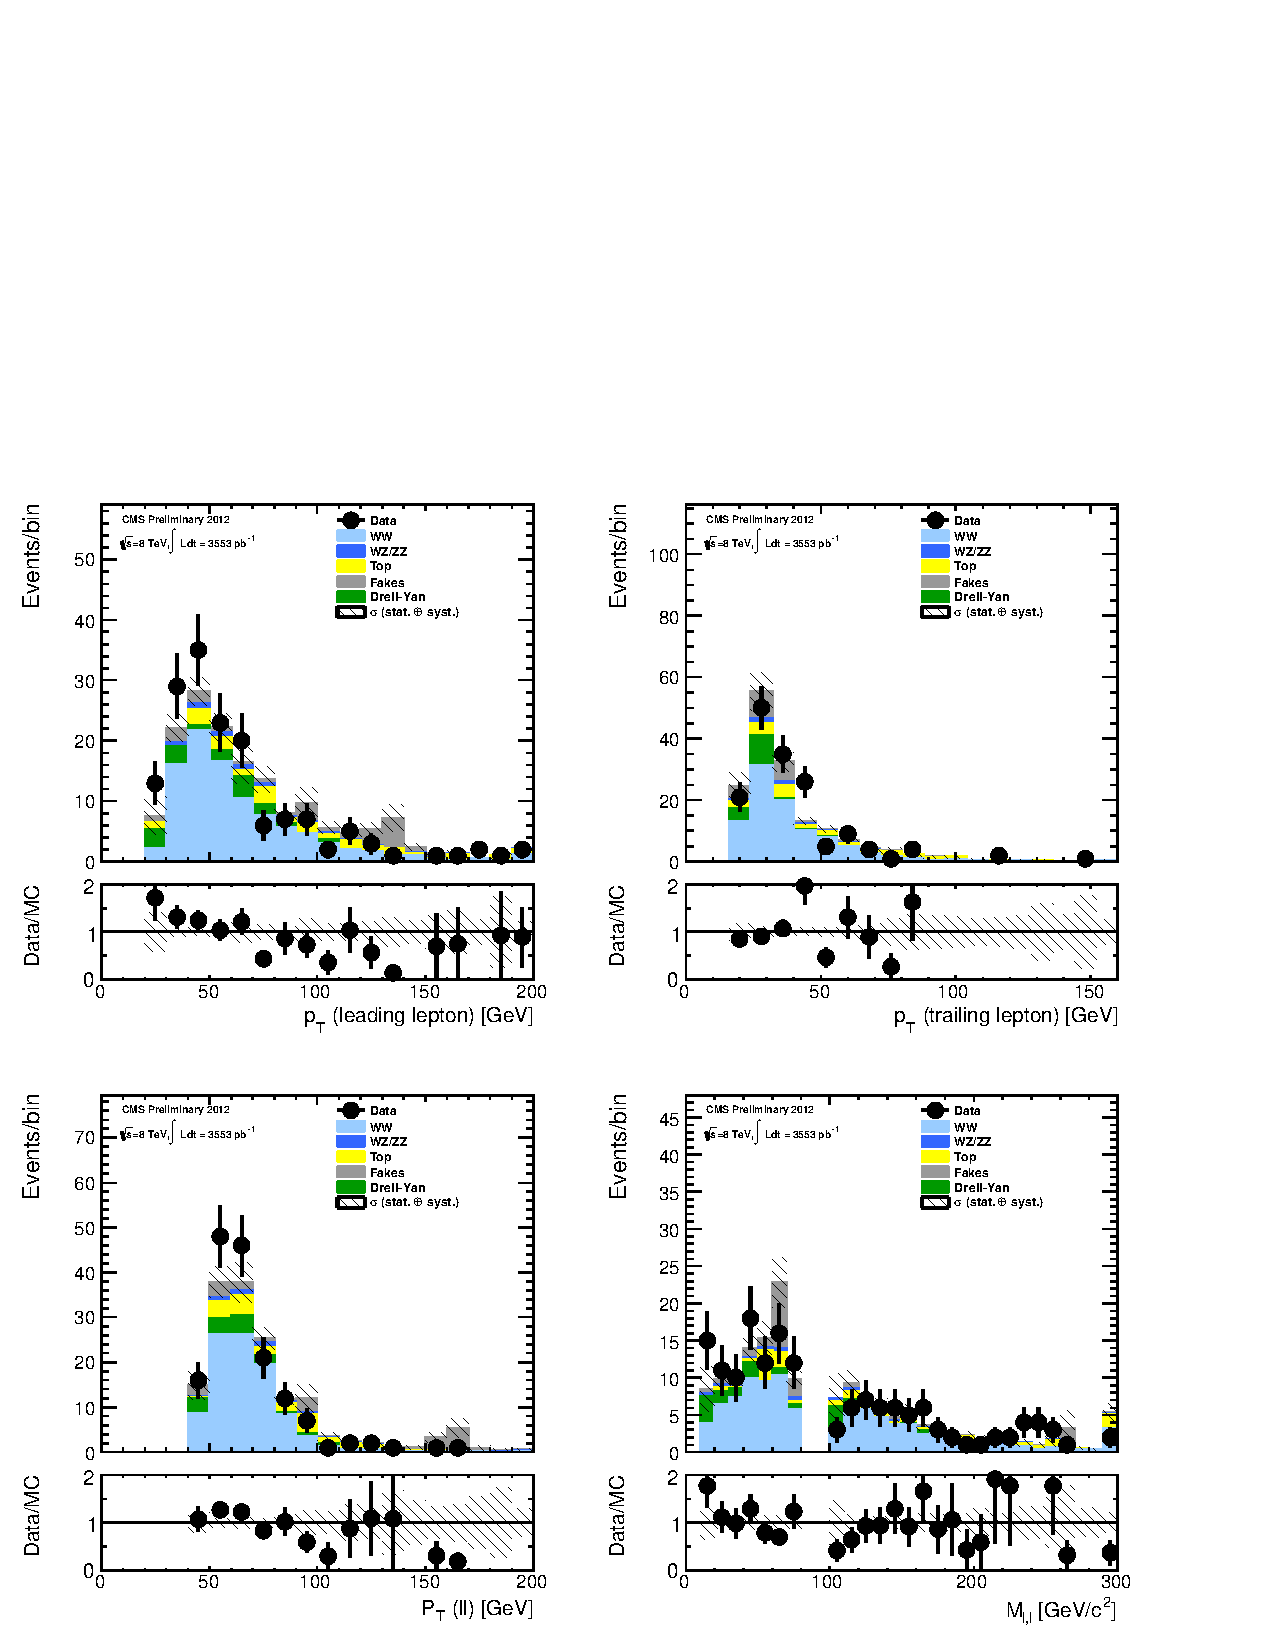
\includegraphics[width=1\textwidth]{figures/ww_analysis20_0_ALL_ee_0j.pdf}
\caption{Kinematic distributions in the $ee$ final state in the 0-jet bin.}
\label{fig:xs_kinematics_ee_0j}
\end{figure}
\begin{figure}[!hbtp]
\centering
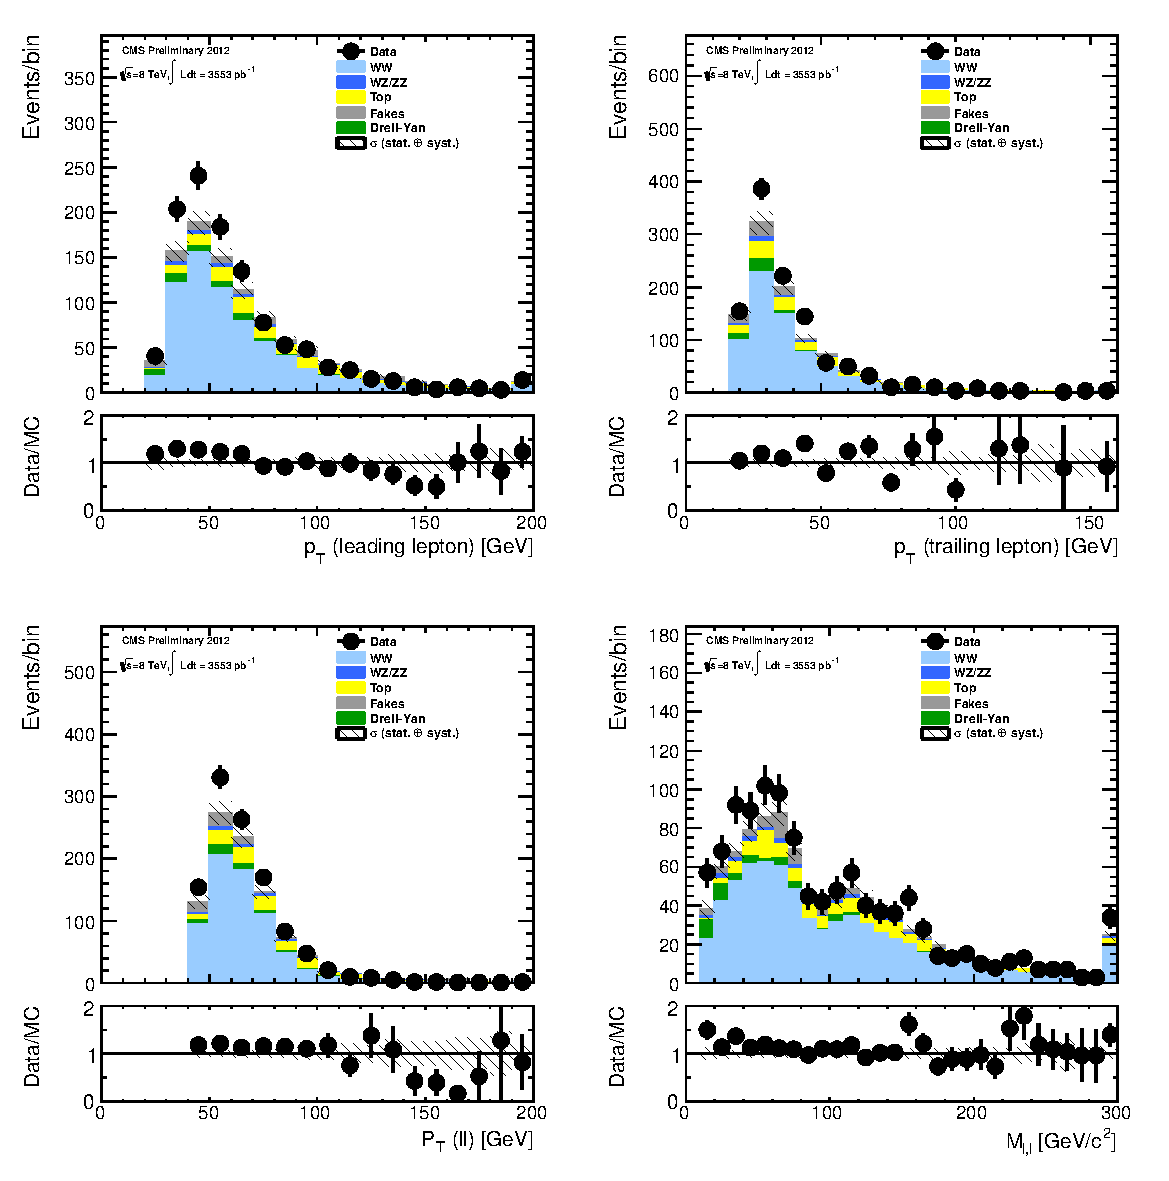
\includegraphics[width=1\textwidth]{figures/ww_analysis20_0_ALL_incl_0j.pdf}
\caption{Kinematic distributions in the inclusive final state in the 0-jet bin.}
\label{fig:xs_kinematics_incl_0j}
\end{figure}

\clearpage
\subsection{Measurements in the 1-Jet bin}

Table~\ref{tab:datayields_wwxsec_1j} shows the expected number of signal and background events,
as well as the signal acceptance and measured cross section in each lepton channel.
Table ~\ref{tab:datayields_wwxsec_1j_incl} shows the results including all lepton channels.
The kinematic distributions of the events selected are shown in Figures \ref{fig:xs_kinematics_mm_1j} - \ref{fig:xs_kinematics_incl_1j}.

\begin{table}[!ht]
{\small
\begin{center}
\begin{tabular}{|l|c|c|c|c|}
\hline
Sample  & mm    & me    & em    & ee    \\ \hline
$qqWW$  & $45.06 \pm 1.26 \pm 3.26 $    & $81.96 \pm 1.78 \pm 5.78 $    & $96.61 \pm 1.91 \pm 6.81 $    & $29.38 \pm 1.03 \pm 2.27 $    \\
$qqWW$  & $2.89 \pm 0.24 \pm 0.89 $ & $4.53 \pm 0.31 \pm 1.39 $ & $4.67 \pm 0.29 \pm 1.44 $ & $2.45 \pm 0.25 \pm 0.75 $ \\
$t\bar{t} + tW$ & $65.46 \pm 5.15 \pm 4.29 $    & $104.14 \pm 6.38 \pm 6.82 $   & $127.45 \pm 7.14 \pm 8.35 $   & $35.37 \pm 3.54 \pm 2.32 $    \\
$W+jets$    & $4.52 \pm 2.71 \pm 1.63 $ & $10.54 \pm 2.86 \pm 3.79 $    & $24.01 \pm 3.45 \pm 8.64 $    & $4.08 \pm 0.76 \pm 1.47 $ \\
$WZ$    & $2.85 \pm 0.13 \pm 0.32 $ & $5.10 \pm 0.18 \pm 0.57 $ & $7.97 \pm 0.23 \pm 0.89 $ & $2.75 \pm 0.13 \pm 0.32 $ \\
$ZZ$    & $1.52 \pm 0.08 \pm 0.15 $ & $0.17 \pm 0.02 \pm 0.02 $ & $0.28 \pm 0.02 \pm 0.03 $ & $0.86 \pm 0.06 \pm 0.09 $ \\
$Z/\gamma*$ & $29.67 \pm 6.23 \pm 5.01 $    & $10.62 \pm 4.04 \pm 1.06 $    & $6.55 \pm 2.06 \pm 0.65 $ & $24.62 \pm 6.58 \pm 4.15 $    \\
$W\gamma*/W+\gamma$ & $0.02 \pm 0.02 \pm 0.01 $ & $1.70 \pm 0.95 \pm 0.51 $ & $6.19 \pm 2.23 \pm 1.86 $ & $4.06 \pm 0.95 \pm 1.22 $ \\
\hline \hline
Total B.    & $104.04 \pm 8.53 \pm 6.80 $   & $132.27 \pm 7.57 \pm 5.14 $   & $172.45 \pm 8.49 \pm 12.21 $  & $71.75 \pm 7.57 \pm 5.14 $    \\ \hline \hline
Total B.+S. & $151.99 \pm 8.63 \pm 7.59 $   & $218.77 \pm 7.78 \pm 7.85 $   & $273.74 \pm 8.71 \pm 14.05 $  & $103.58 \pm 7.64 \pm 5.66 $   \\ \hline \hline
Data    & $155$     & $213$     & $267$     & $115$     \\ \hline \hline
Acceptance ( \% )   & $0.23 \pm 0.02    $& $0.41 \pm 0.03   $& $0.48 \pm 0.04   $& $0.15 \pm 0.01   $\\
Cross Section ( pb )    & $60.70 \pm 14.83 \pm 13.86$   & $53.30 \pm 9.64 \pm 7.32$     & $53.31 \pm 9.21 \pm 9.35$     & $77.60 \pm 19.24 \pm 17.66$   \\ \hline
\end{tabular}
\caption{Summary of yields for 1-jet channel.Uncertainties on yields and cross sections are $\mathrm{(stat.)} \pm \mathrm{(syst.)}$. The systematic uncertainty on the cross section does not include the luminosity}
\label{tab:datayields_wwxsec_1j}
\end{center}}
\end{table}
\begin{table}[!ht]
{\small
\begin{center}
\begin{tabular}{|l|c|c|c|c|}
\hline
Sample  & incl  \\ \hline
$qqWW$  & $253.02 \pm 3.08 \pm 18.11 $  \\
$qqWW$  & $14.54 \pm 0.55 \pm 4.47 $    \\
$t\bar{t} + tW$ & $332.43 \pm 11.43 \pm 21.77 $ \\
$W+jets$    & $43.15 \pm 5.29 \pm 15.53 $   \\
$WZ$    & $18.67 \pm 0.34 \pm 2.10 $    \\
$ZZ$    & $2.83 \pm 0.11 \pm 0.28 $ \\
$Z/\gamma*$ & $71.46 \pm 10.13 \pm 9.32 $   \\
$W\gamma*/W+\gamma$ & $11.97 \pm 2.61 \pm 3.59 $    \\
\hline \hline
Total B.    & $480.51 \pm 16.38 \pm 28.63 $ \\ \hline \hline
Total B.+S. & $748.07 \pm 16.68 \pm 34.17 $ \\ \hline \hline
Data    & $750$     \\ \hline \hline
Acceptance ( \% )   & $1.26 \pm 0.10    $\\
Cross Section ( pb )    & $57.52 \pm 5.85 \pm 8.37$     \\ \hline
\end{tabular}
\caption{Summary of yields for 1-jet channel.Uncertainties on yields and cross sections are $\mathrm{(stat.)} \pm \mathrm{(syst.)}$. The systematic uncertainty on the cross section does not include the luminosity}
\label{tab:datayields_wwxsec_1j_incl}
\end{center}}
\end{table}

\begin{figure}[!hbtp]
\centering
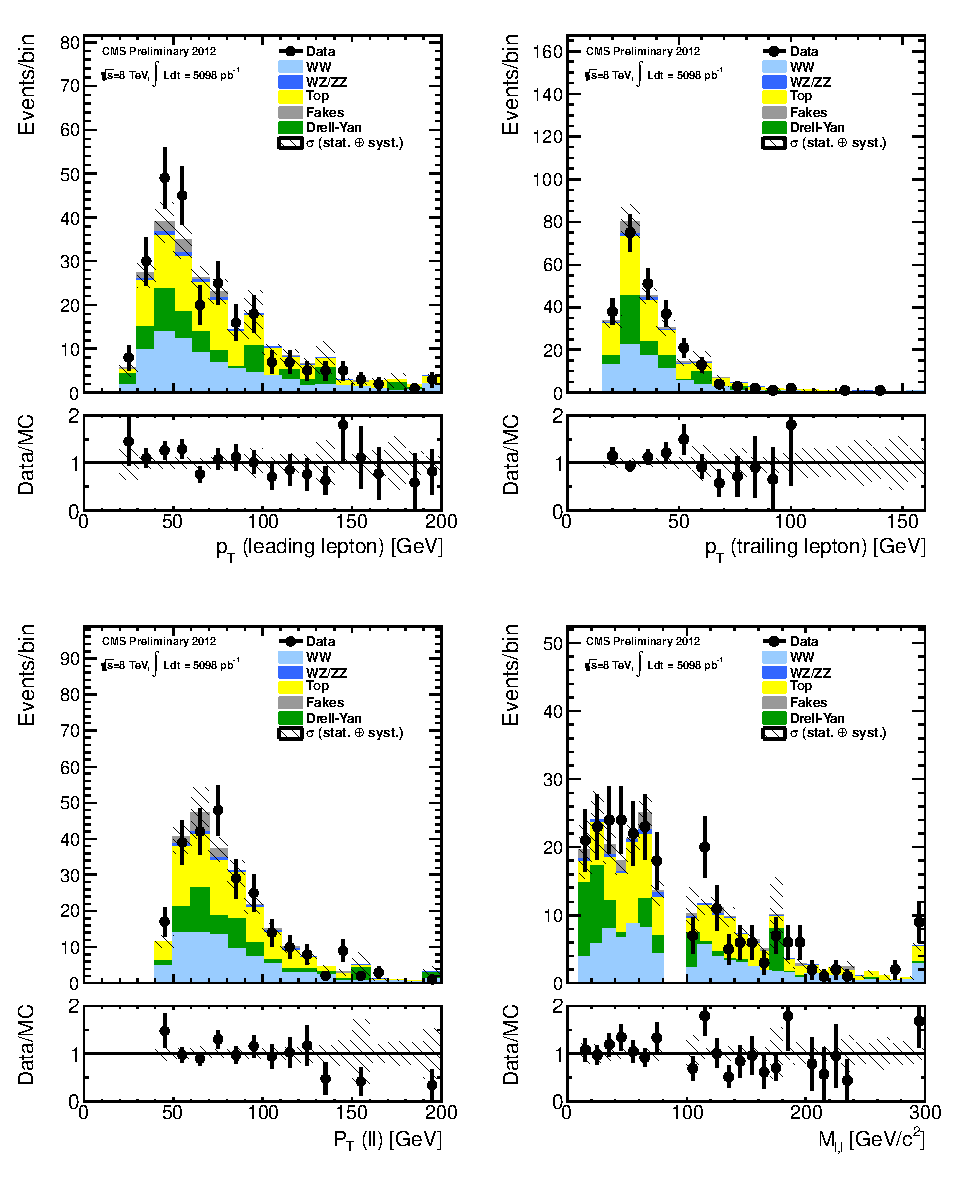
\includegraphics[width=1\textwidth]{figures/ww_analysis20_0_ALL_mm_1j.pdf}
\caption{Kinematic distributions in the $\mu\mu$ final state in the 1-jet bin.}
\label{fig:xs_kinematics_mm_1j}
\end{figure}
\begin{figure}[!hbtp]
\centering
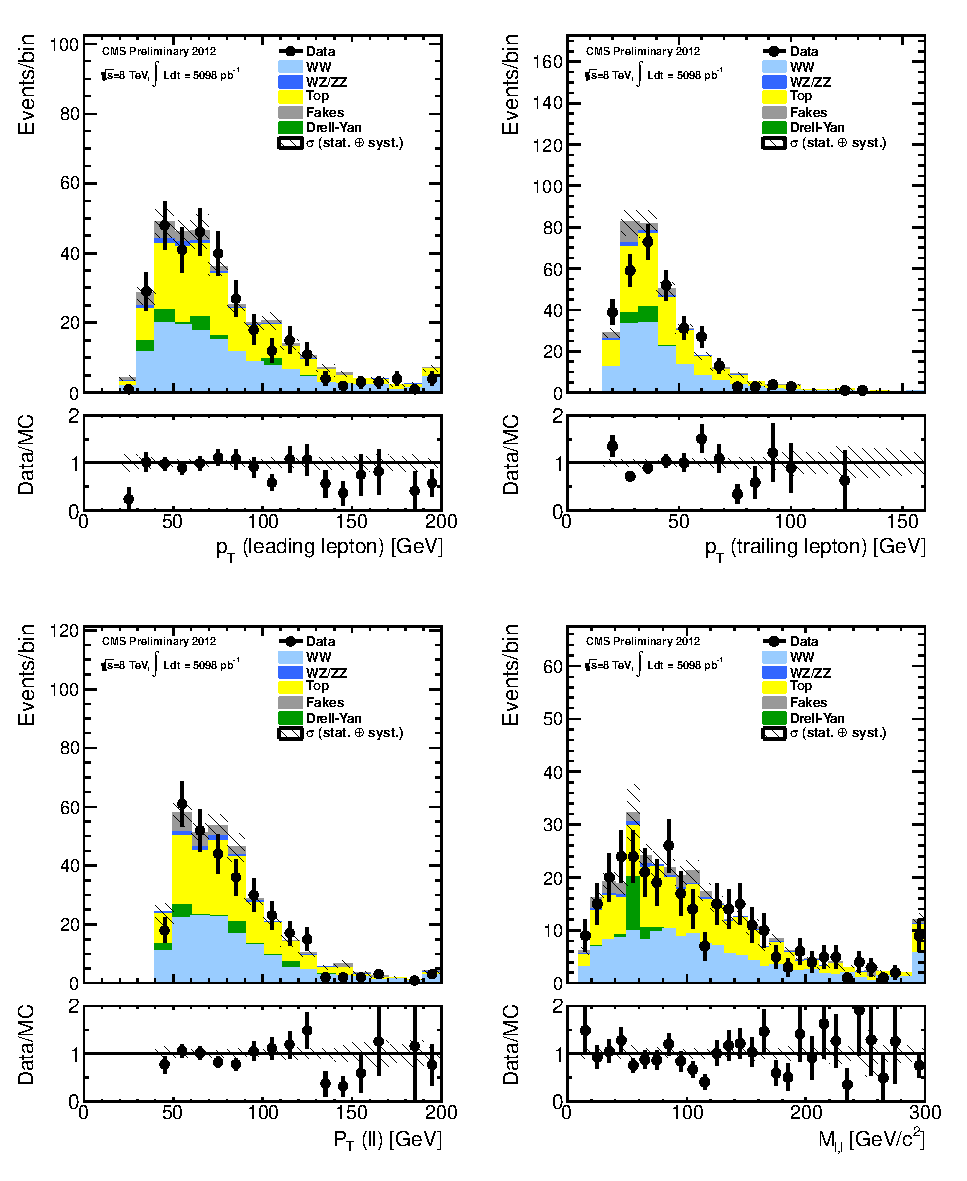
\includegraphics[width=1\textwidth]{figures/ww_analysis20_0_ALL_me_1j.pdf}
\caption{Kinematic distributions in the $\mu e$ final state in the 1-jet bin.}
\label{fig:xs_kinematics_me_1j}
\end{figure}
\begin{figure}[!hbtp]
\centering
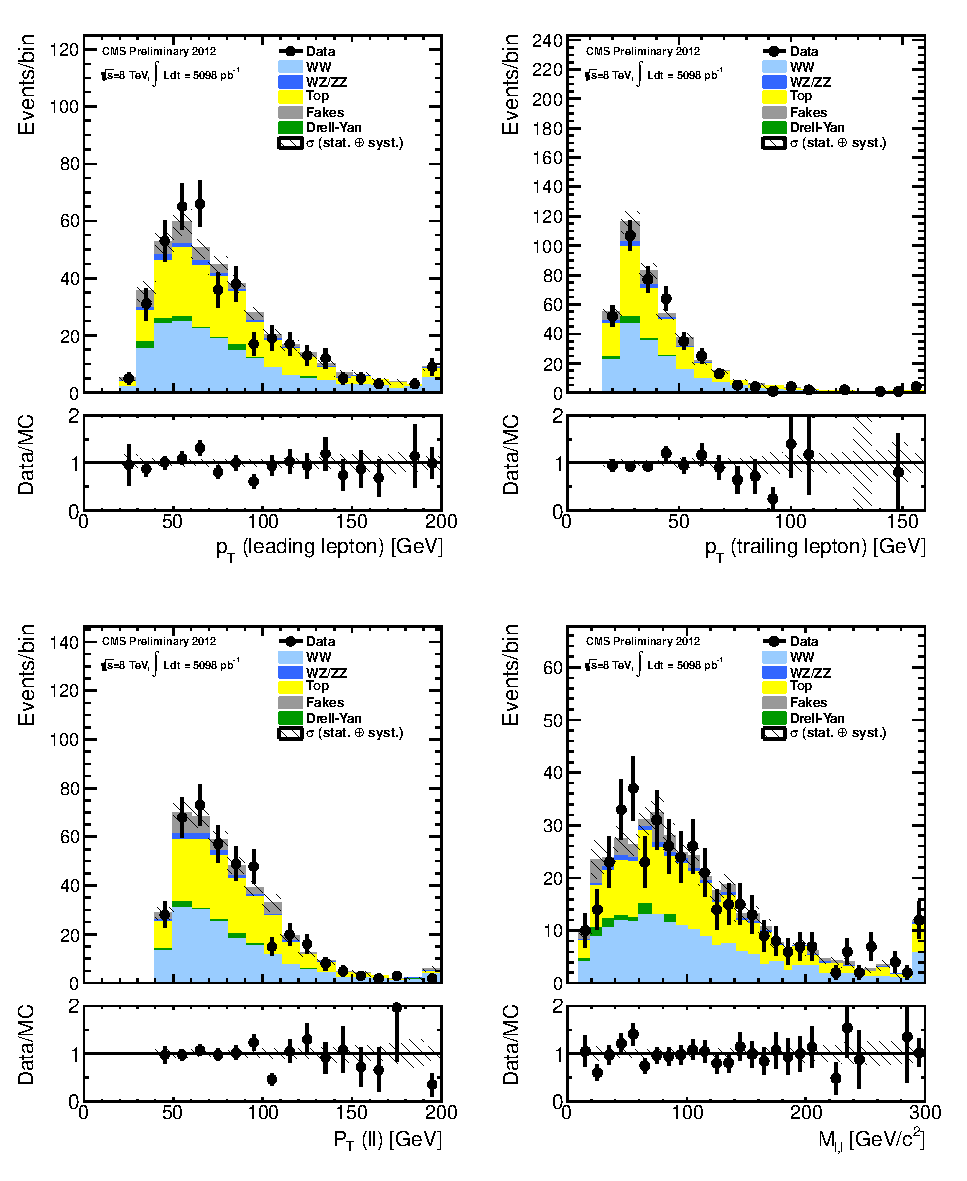
\includegraphics[width=1\textwidth]{figures/ww_analysis20_0_ALL_em_1j.pdf}
\caption{Kinematic distributions in the $e\mu$ final state in the 1-jet bin.}
\label{fig:xs_kinematics_em_1j}
\end{figure}
\begin{figure}[!hbtp]
\centering
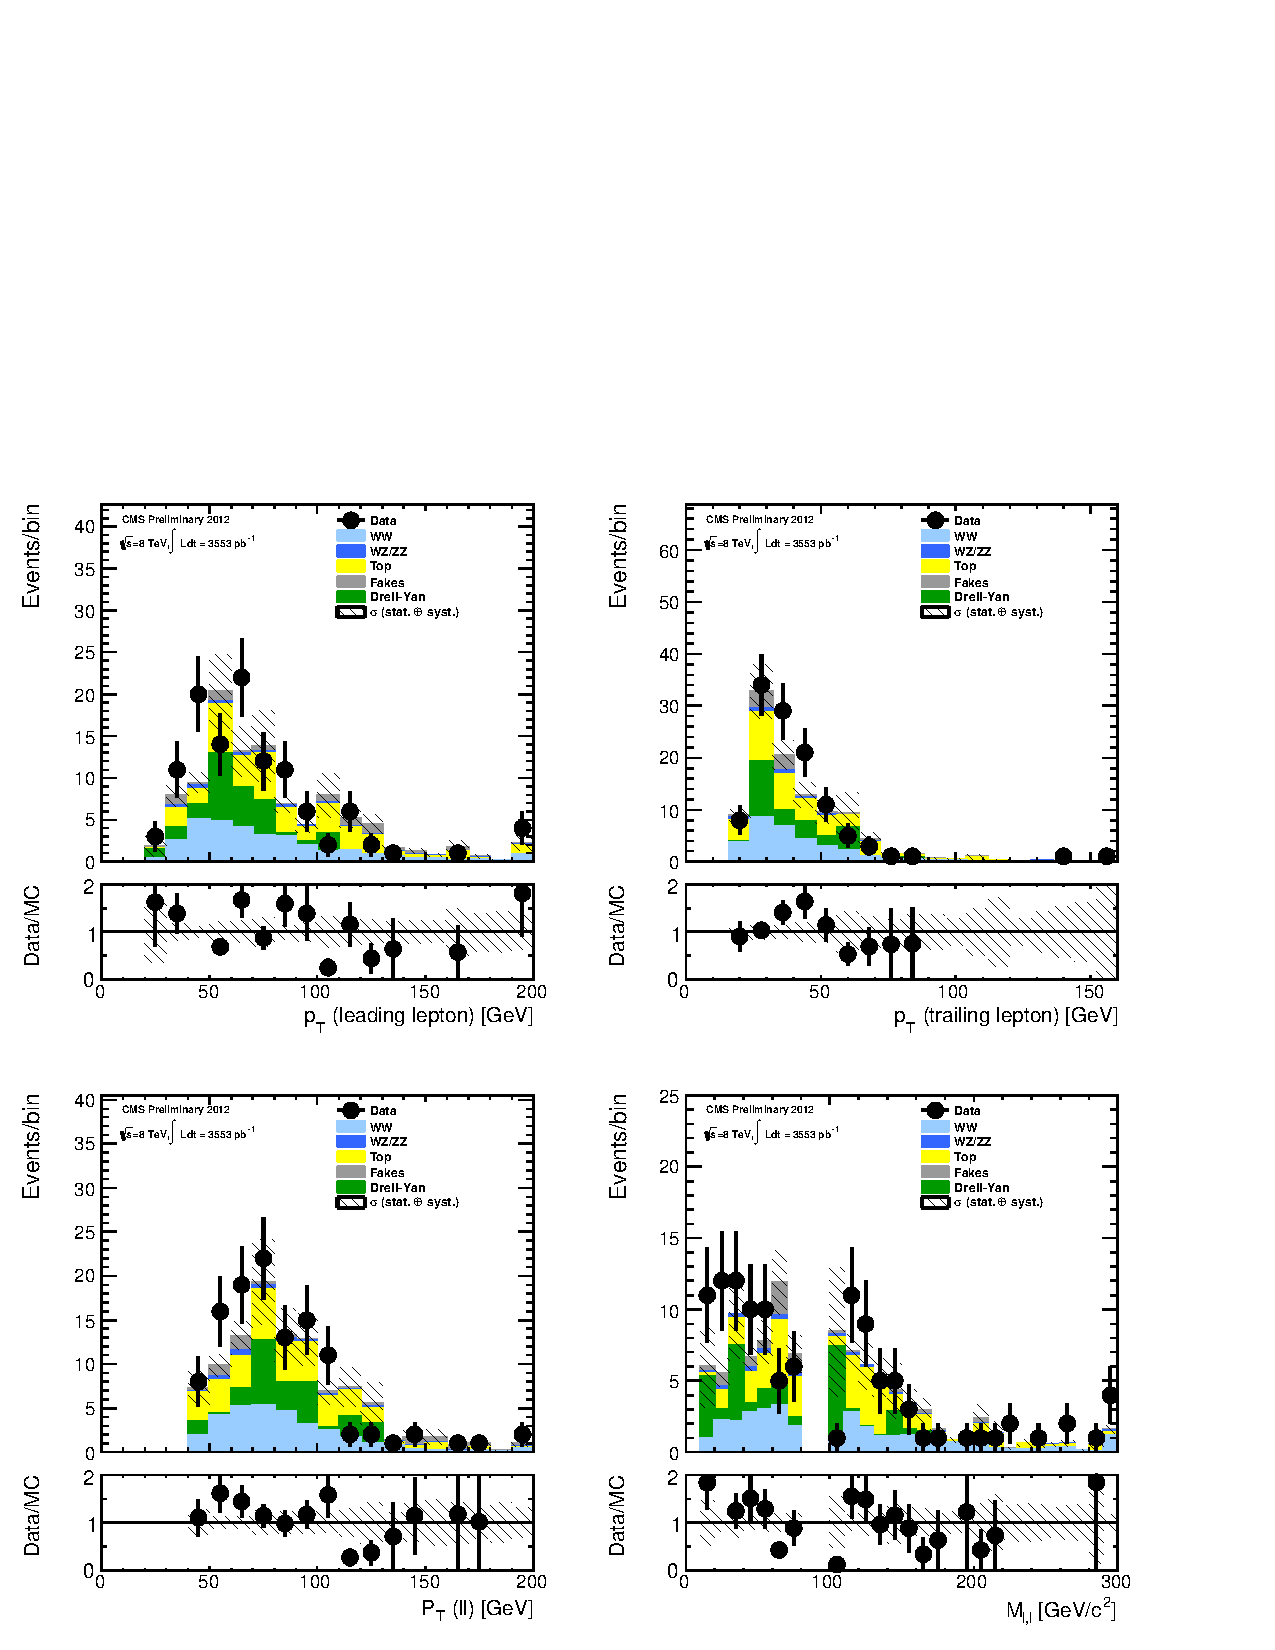
\includegraphics[width=1\textwidth]{figures/ww_analysis20_0_ALL_ee_1j.pdf}
\caption{Kinematic distributions in the $ee$ final state in the 1-jet bin.}
\label{fig:xs_kinematics_ee_1j}
\end{figure}
\begin{figure}[!hbtp]
\centering
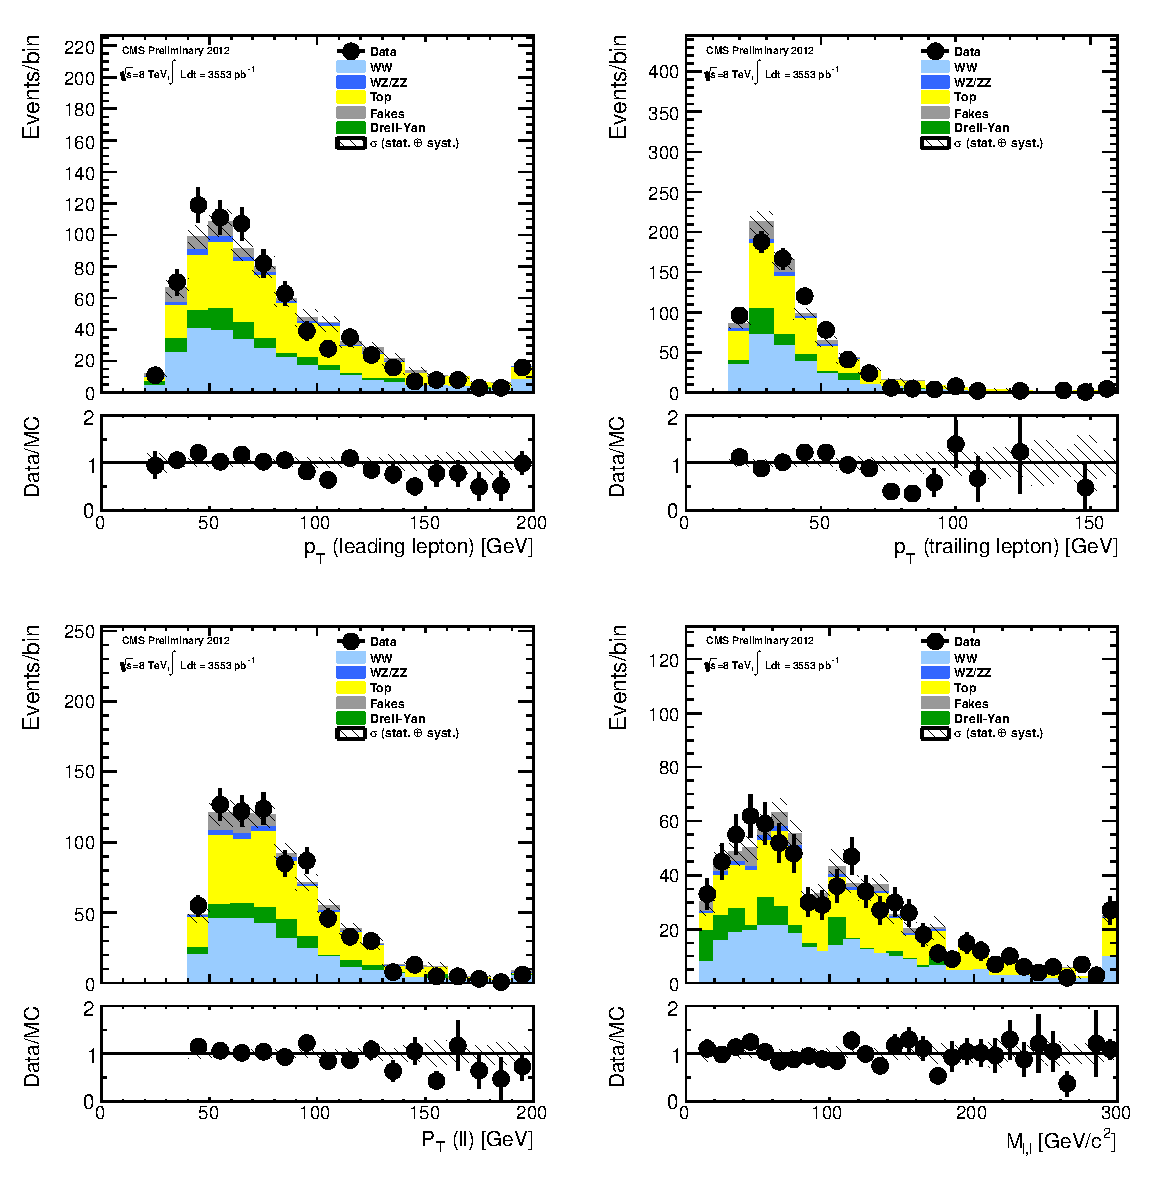
\includegraphics[width=1\textwidth]{figures/ww_analysis20_0_ALL_incl_1j.pdf}
\caption{Kinematic distributions in the inclusive final state in the 1-jet bin.}
\label{fig:xs_kinematics_incl_1j}
\end{figure}

\clearpage
\subsection{Measurements in the 2-Jet bin}

Table~\ref{tab:datayields_wwxsec_2j} shows the expected number of signal and background events,
as well as the signal acceptance and measured cross section in each lepton channel.
Table ~\ref{tab:datayields_wwxsec_2j_incl} shows the results including all lepton channels.
The kinematic distributions of the events selected are shown in Figures \ref{fig:xs_kinematics_mm_2j} - \ref{fig:xs_kinematics_incl_2j}.
\begin{table}[!ht]
{\small
\begin{center}
\begin{tabular}{|l|c|c|c|c|}
\hline
Sample  & mm    & me    & em    & ee    \\ \hline
$qqWW$  & $20.94 \pm 0.86 \pm 1.52 $    & $31.47 \pm 1.07 \pm 2.22 $    & $37.46 \pm 1.21 \pm 2.64 $    & $13.86 \pm 0.71 \pm 1.07 $    \\
$qqWW$  & $0.39 \pm 0.07 \pm 0.12 $ & $0.92 \pm 0.14 \pm 0.28 $ & $0.95 \pm 0.15 \pm 0.29 $ & $0.52 \pm 0.11 \pm 0.16 $ \\
$t\bar{t} + tW$ & $100.94 \pm 6.69 \pm 6.26 $   & $120.38 \pm 6.81 \pm 7.46 $   & $138.82 \pm 7.33 \pm 8.61 $   & $56.99 \pm 4.83 \pm 3.53 $    \\
$W+jets$    & $2.31 \pm 2.81 \pm 0.83 $ & $8.24 \pm 2.35 \pm 2.97 $ & $7.06 \pm 2.92 \pm 2.54 $ & $1.52 \pm 0.74 \pm 0.55 $ \\
$WZ$    & $1.98 \pm 0.11 \pm 0.22 $ & $2.60 \pm 0.13 \pm 0.29 $ & $3.70 \pm 0.15 \pm 0.41 $ & $1.97 \pm 0.11 \pm 0.23 $ \\
$ZZ$    & $0.76 \pm 0.07 \pm 0.07 $ & $0.08 \pm 0.01 \pm 0.01 $ & $0.19 \pm 0.03 \pm 0.02 $ & $0.41 \pm 0.04 \pm 0.04 $ \\
$Z/\gamma*$ & $54.75 \pm 7.65 \pm 9.64 $    & $9.11 \pm 3.74 \pm 0.91 $ & $6.48 \pm 2.69 \pm 0.65 $ & $43.18 \pm 9.65 \pm 7.60 $    \\
$W\gamma*/W+\gamma$ & $0.00 \pm 0.00 \pm 0.00 $ & $0.40 \pm 0.33 \pm 0.12 $ & $0.90 \pm 0.72 \pm 0.27 $ & $0.87 \pm 0.50 \pm 0.26 $ \\
\hline \hline
Total B.    & $160.74 \pm 10.55 \pm 11.52 $ & $140.81 \pm 10.83 \pm 8.41 $  & $157.16 \pm 8.37 \pm 9.01 $   & $104.94 \pm 10.83 \pm 8.41 $  \\ \hline \hline
Total B.+S. & $182.08 \pm 10.58 \pm 11.62 $ & $173.20 \pm 10.88 \pm 8.70 $  & $195.57 \pm 8.46 \pm 9.40 $   & $119.31 \pm 10.85 \pm 8.48 $  \\ \hline \hline
Data    & $196$     & $179$     & $216$     & $110$     \\ \hline \hline
Acceptance ( \% )   & $0.10 \pm 0.01    $& $0.15 \pm 0.01   $& $0.18 \pm 0.01   $& $0.07 \pm 0.01   $\\
Cross Section ( pb )    & $94.37 \pm 37.47 \pm 42.48$   & $67.34 \pm 23.59 \pm 24.74$   & $87.50 \pm 21.85 \pm 19.51$   & $20.11 \pm 41.66 \pm 54.49$   \\ \hline
\end{tabular}
\caption{Summary of yields for 2-jet channel.Uncertainties on yields and cross sections are $\mathrm{(stat.)} \pm \mathrm{(syst.)}$. The systematic uncertainty on the cross section does not include the luminosity}
\label{tab:datayields_wwxsec_2j}
\end{center}}
\end{table}
\begin{table}[!ht]
{\small
\begin{center}
\begin{tabular}{|l|c|c|c|c|}
\hline
Sample  & incl  \\ \hline
$qqWW$  & $103.73 \pm 1.96 \pm 7.44 $   \\
$qqWW$  & $2.78 \pm 0.24 \pm 0.85 $ \\
$t\bar{t} + tW$ & $417.14 \pm 12.97 \pm 25.86 $ \\
$W+jets$    & $19.14 \pm 4.74 \pm 6.89 $    \\
$WZ$    & $10.24 \pm 0.25 \pm 1.16 $    \\
$ZZ$    & $1.44 \pm 0.08 \pm 0.14 $ \\
$Z/\gamma*$ & $113.51 \pm 13.15 \pm 17.31 $ \\
$W\gamma*/W+\gamma$ & $2.18 \pm 0.94 \pm 0.65 $ \\
\hline \hline
Total B.    & $563.65 \pm 19.09 \pm 31.90 $ \\ \hline \hline
Total B.+S. & $670.15 \pm 19.20 \pm 32.77 $ \\ \hline \hline
Data    & $701$     \\ \hline \hline
Acceptance ( \% )   & $0.50 \pm 0.04    $\\
Cross Section ( pb )    & $73.65 \pm 14.20 \pm 20.76$   \\ \hline
\end{tabular}
\caption{Summary of yields for 2-jet channel.Uncertainties on yields and cross sections are $\mathrm{(stat.)} \pm \mathrm{(syst.)}$. The systematic uncertainty on the cross section does not include the luminosity}
\label{tab:datayields_wwxsec_2j_incl}
\end{center}}
\end{table}

\begin{figure}[!hbtp]
\centering
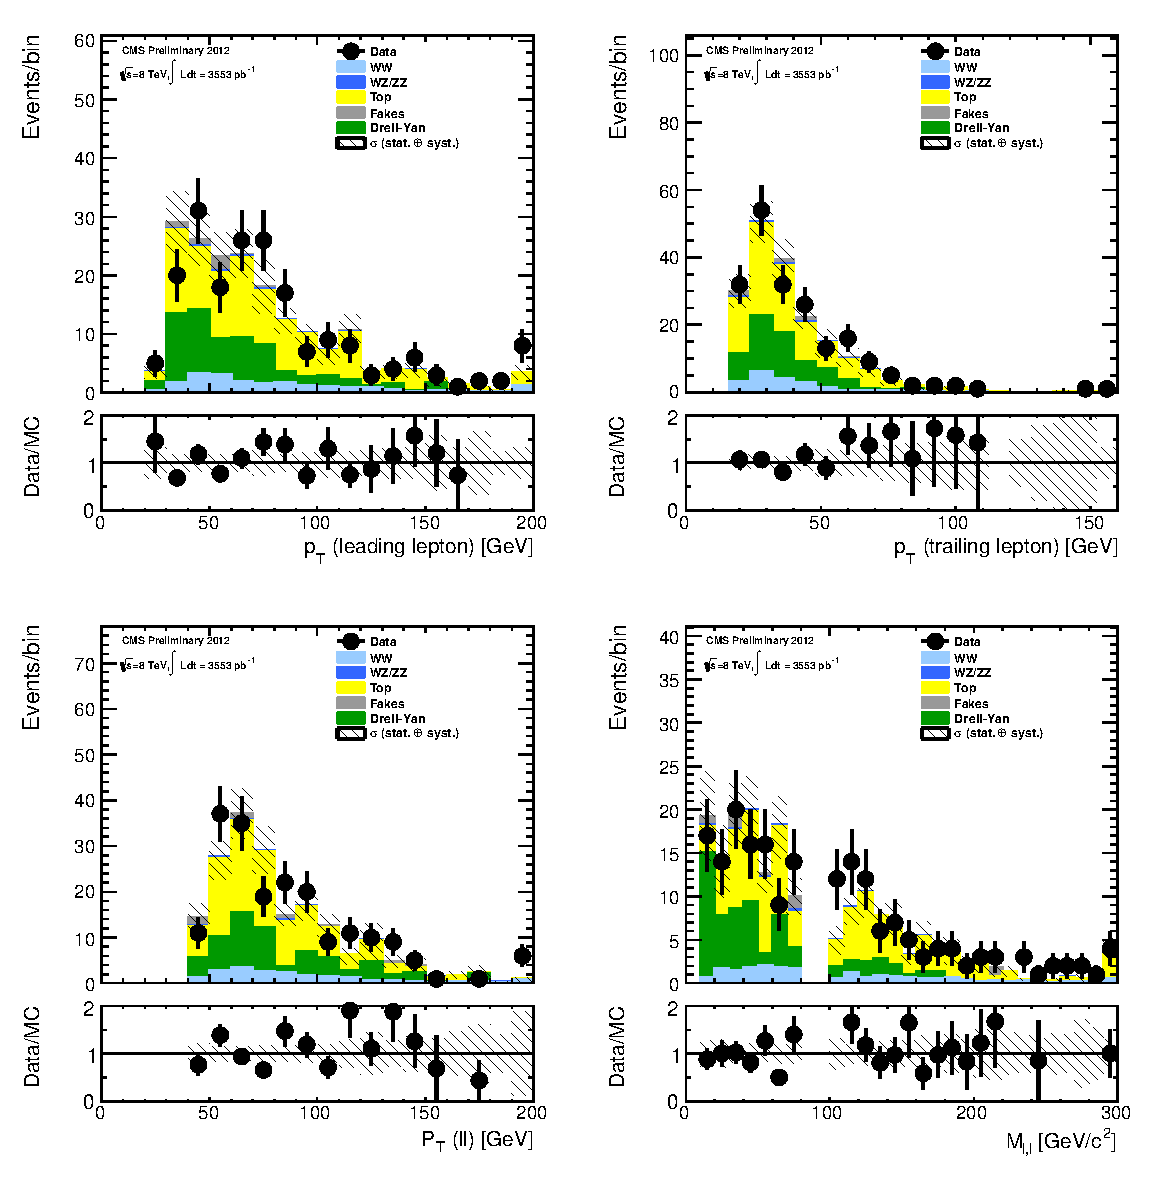
\includegraphics[width=1\textwidth]{figures/ww_analysis20_0_ALL_mm_2j.pdf}
\caption{Kinematic distributions in the $\mu\mu$ final state in the 2-jet bin.}
\label{fig:xs_kinematics_mm_2j}
\end{figure}
\begin{figure}[!hbtp]
\centering
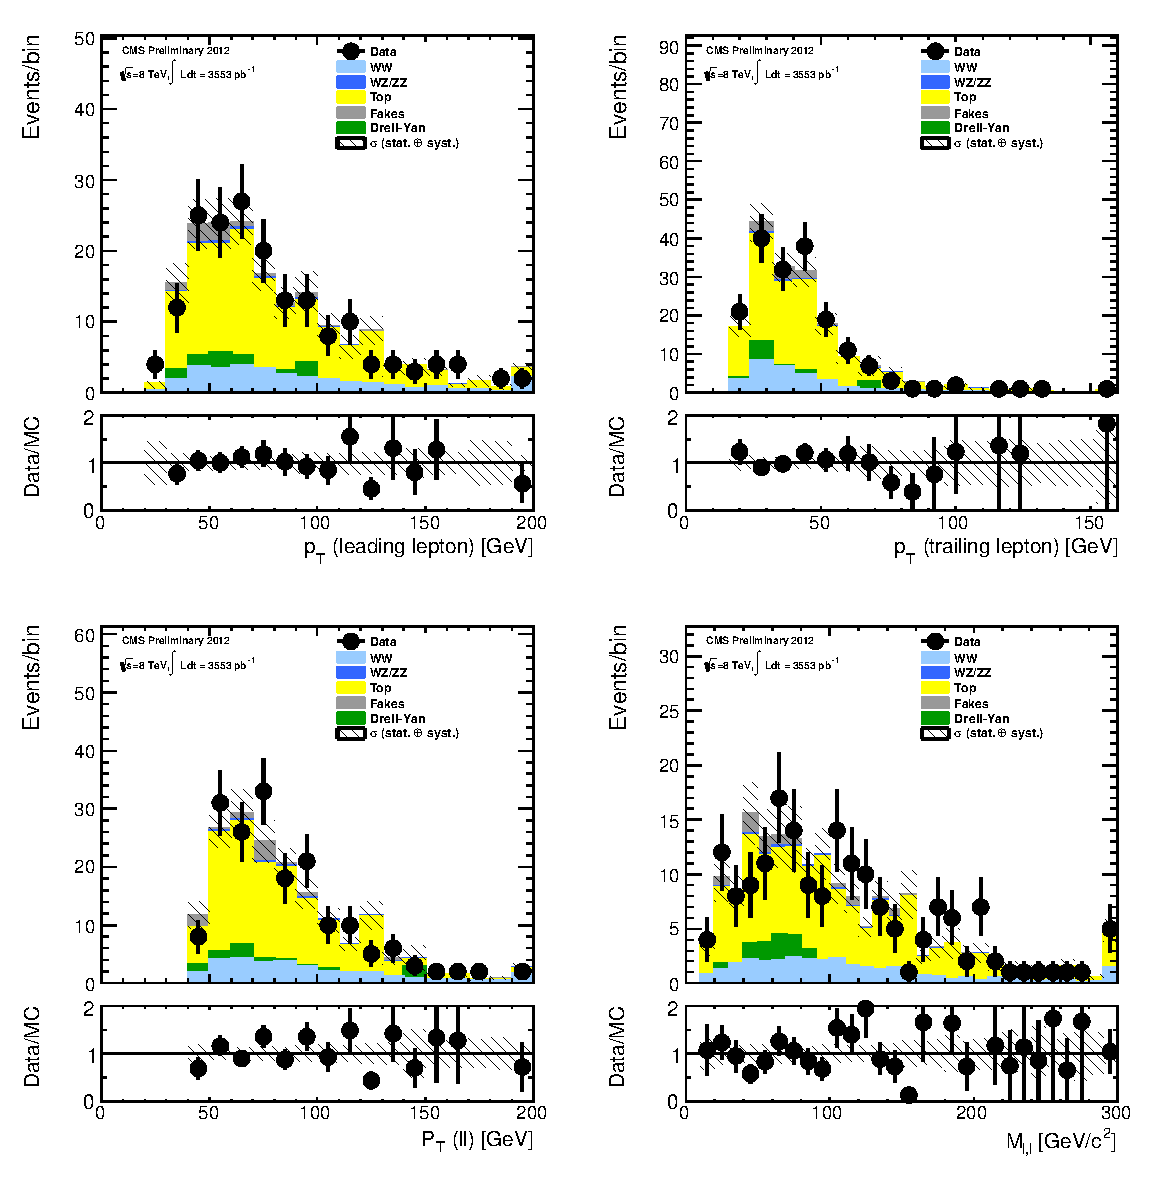
\includegraphics[width=1\textwidth]{figures/ww_analysis20_0_ALL_me_2j.pdf}
\caption{Kinematic distributions in the $\mu e$ final state in the 2-jet bin.}
\label{fig:xs_kinematics_me_2j}
\end{figure}
\begin{figure}[!hbtp]
\centering
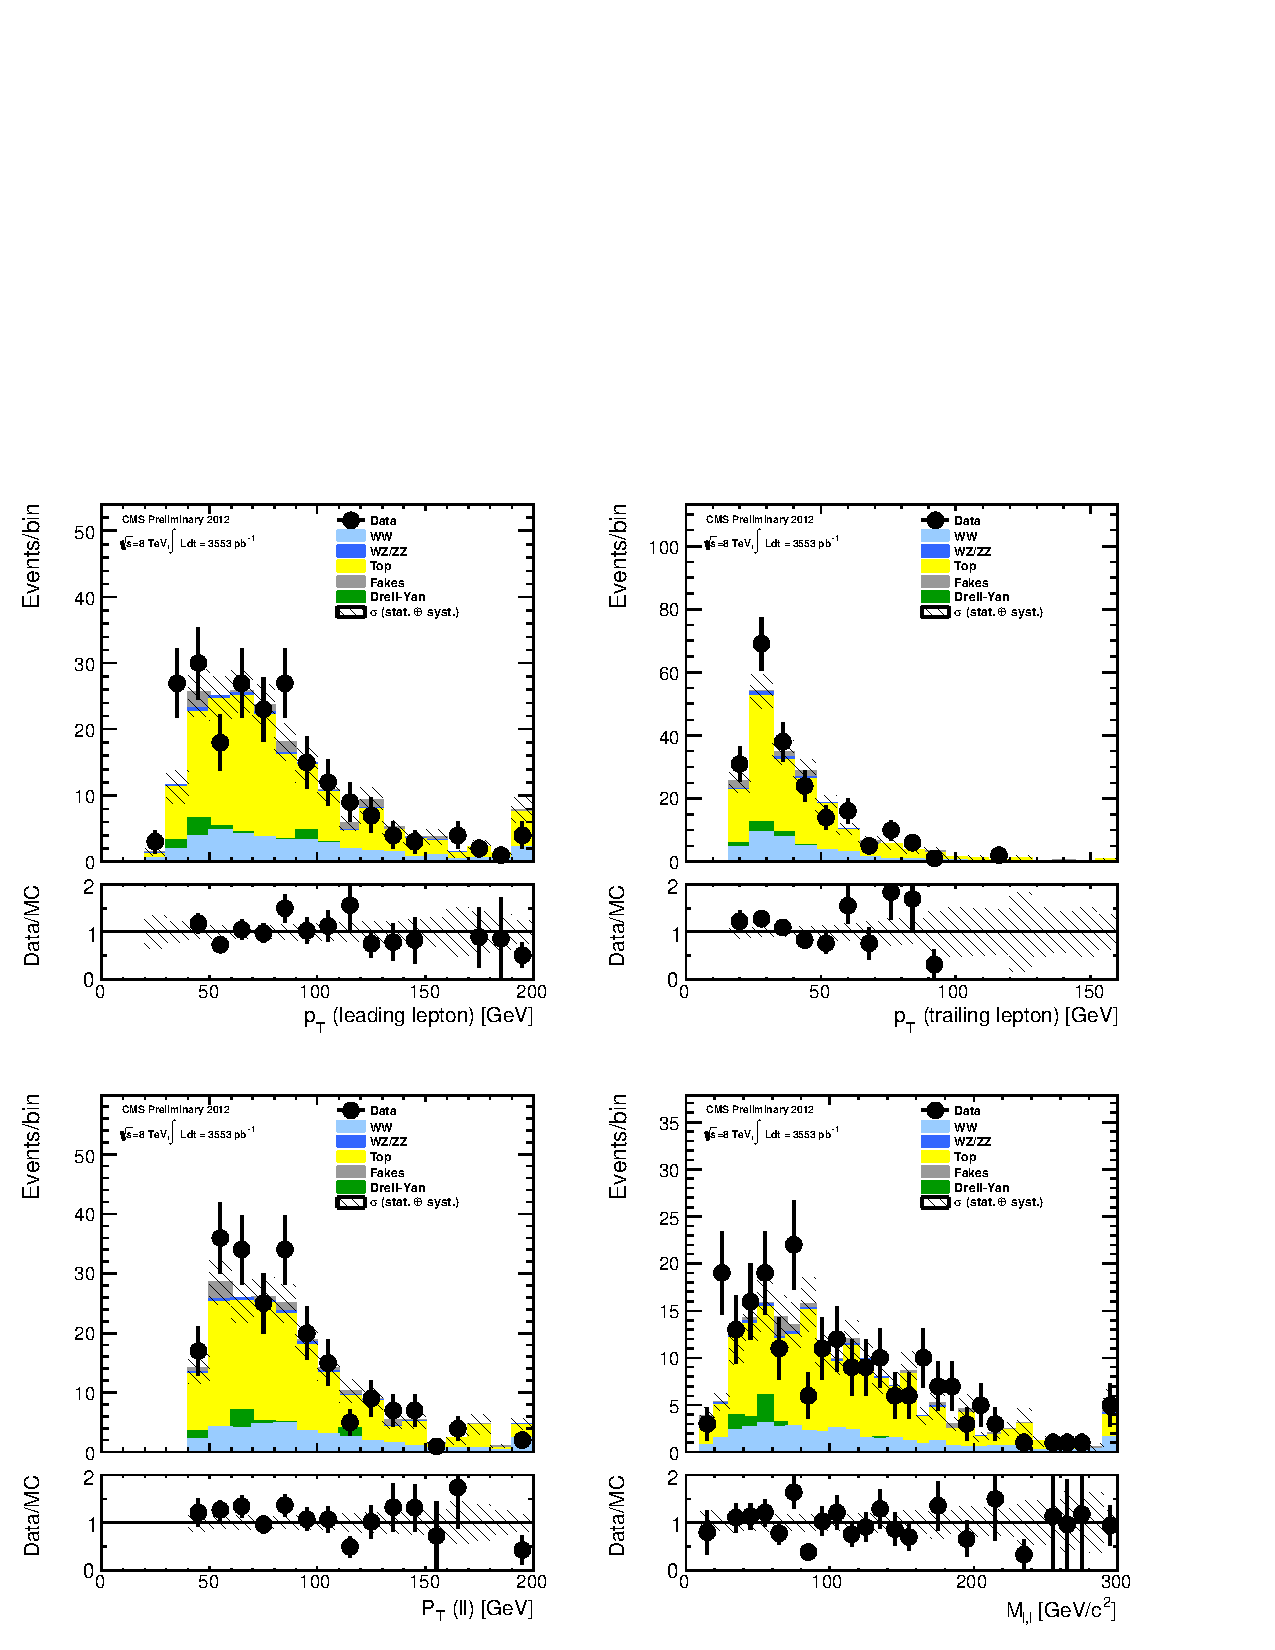
\includegraphics[width=1\textwidth]{figures/ww_analysis20_0_ALL_em_2j.pdf}
\caption{Kinematic distributions in the $e\mu$ final state in the 2-jet bin.}
\label{fig:xs_kinematics_em_2j}
\end{figure}
\begin{figure}[!hbtp]
\centering
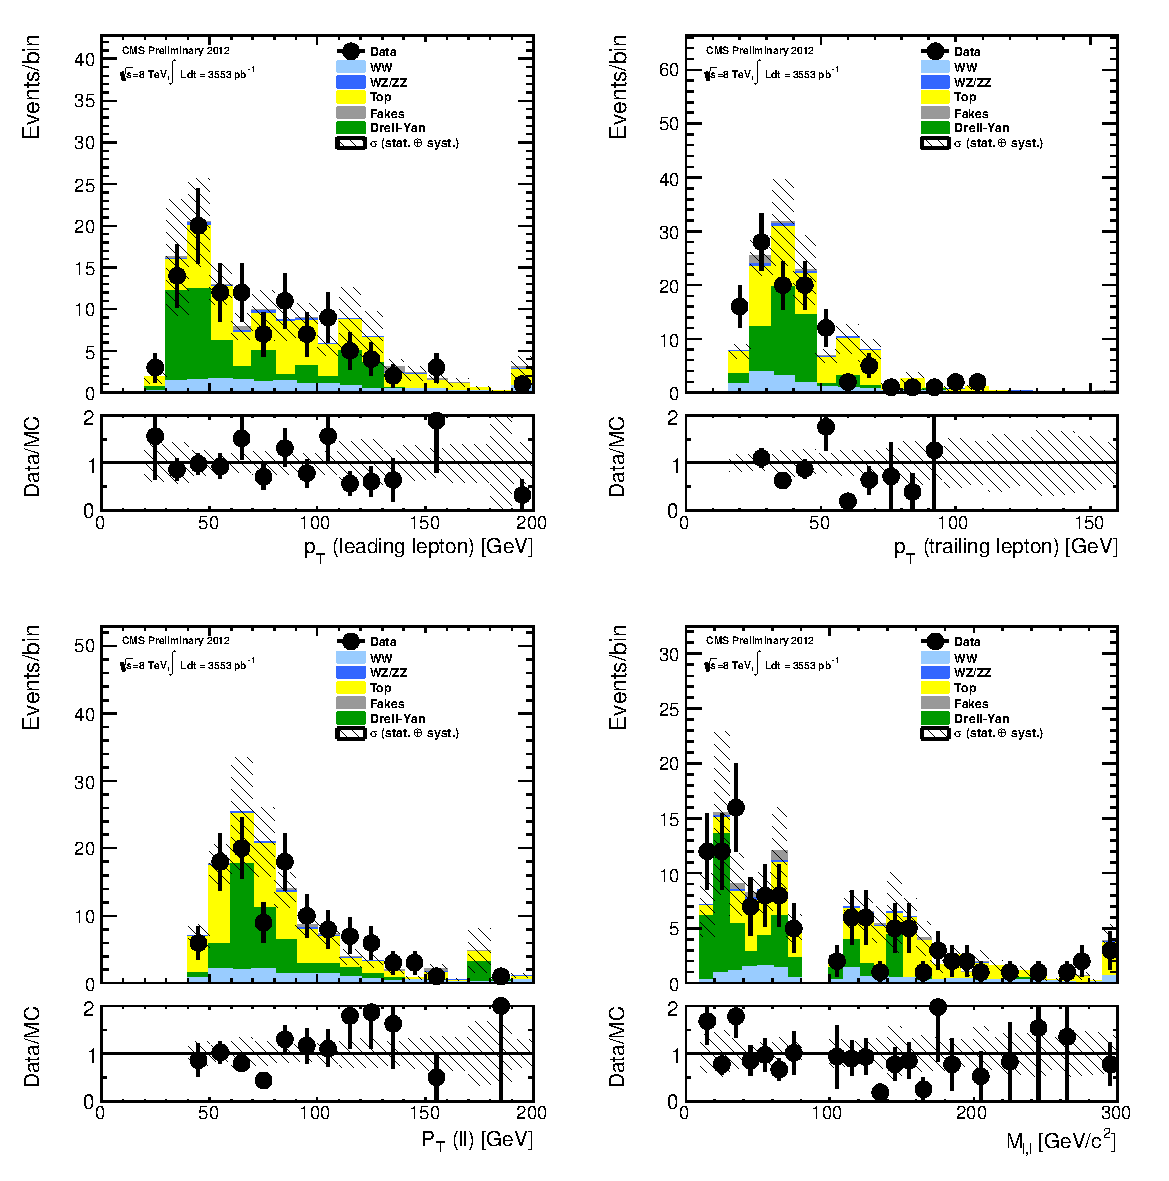
\includegraphics[width=1\textwidth]{figures/ww_analysis20_0_ALL_ee_2j.pdf}
\caption{Kinematic distributions in the $ee$ final state in the 2-jet bin.}
\label{fig:xs_kinematics_ee_2j}
\end{figure}
\begin{figure}[!hbtp]
\centering
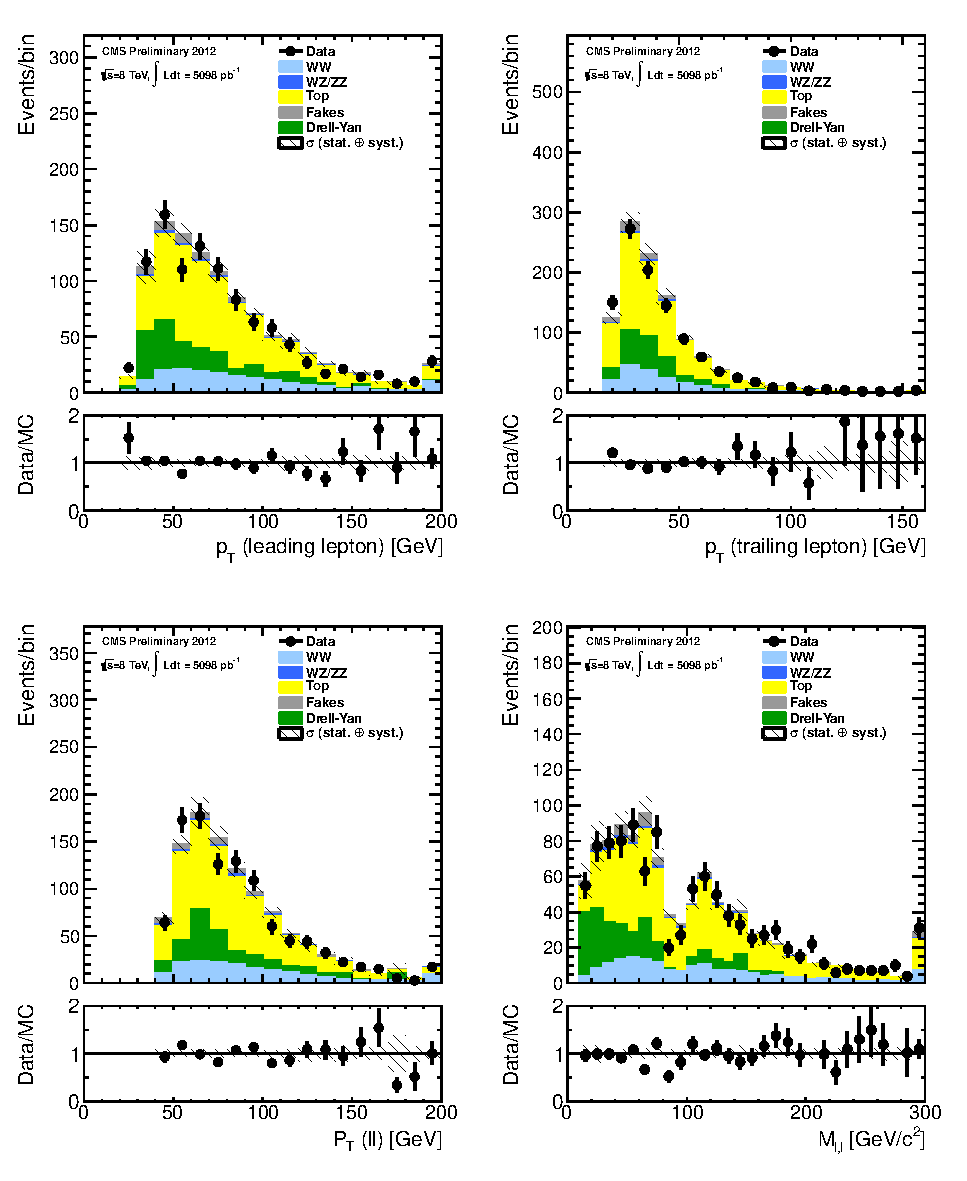
\includegraphics[width=1\textwidth]{figures/ww_analysis20_0_ALL_incl_2j.pdf}
\caption{Kinematic distributions in the inclusive final state in the 2-jet bin.}
\label{fig:xs_kinematics_incl_2j}
\end{figure}

\clearpage
\subsection{Summary}

The measurements in each jet bin and lepton channel are sumamrised in
Table \ref{tab:xs_summary}.  These are shown graphically 
in Figure \ref{fig:xs_summary_figure}.

\begin{table}[!ht]
\begin{center}
\begin{tabular}{|l|c|c|c|}
\hline
Channel              & 0-jet & 1-jet & 2-jet \\ \hline
$\sigma_{\mu\mu}$   &  $64.56\pm5.93\pm6.73\pm3.23$  & $60.70\pm14.83\pm13.86\pm3.03$ & $94.37\pm37.47\pm42.48\pm4.72$ \\
$\sigma_{\mu e}$   &  $72.31\pm5.02\pm6.29\pm3.62$  & $53.30\pm9.64\pm7.32\pm2.67$ & $67.34\pm23.59\pm24.74\pm3.37$ \\
$\sigma_{e \mu}$   &  $72.81\pm4.69\pm6.69\pm3.64$  & $53.31\pm9.21\pm9.35\pm2.67$ & $87.50\pm21.85\pm19.51\pm4.37$ \\
$\sigma_{ee}$   &  $56.03\pm7.40\pm7.52\pm2.80$  & $77.60\pm19.24\pm17.66\pm3.88$ & $20.11\pm41.66\pm54.49\pm1.01$ \\
\hline \hline
$\sigma_{tot.}$   &  $68.51\pm2.75\pm6.28\pm3.43$  & $57.52\pm5.85\pm8.37\pm2.88$ & $73.65\pm14.20\pm20.76\pm3.68$ \\
\hline
\end{tabular}
\caption{Summary of cross section results.  Uncertainties are $\mathrm{(stat.)} \pm \mathrm{(syst.)} \pm\mathrm{(lumi.)~pb}$.}
\label{tab:xs_summary}
\end{center}
\end{table}
\vspace{30pt}
\begin{figure}[!hbtp]
\centering
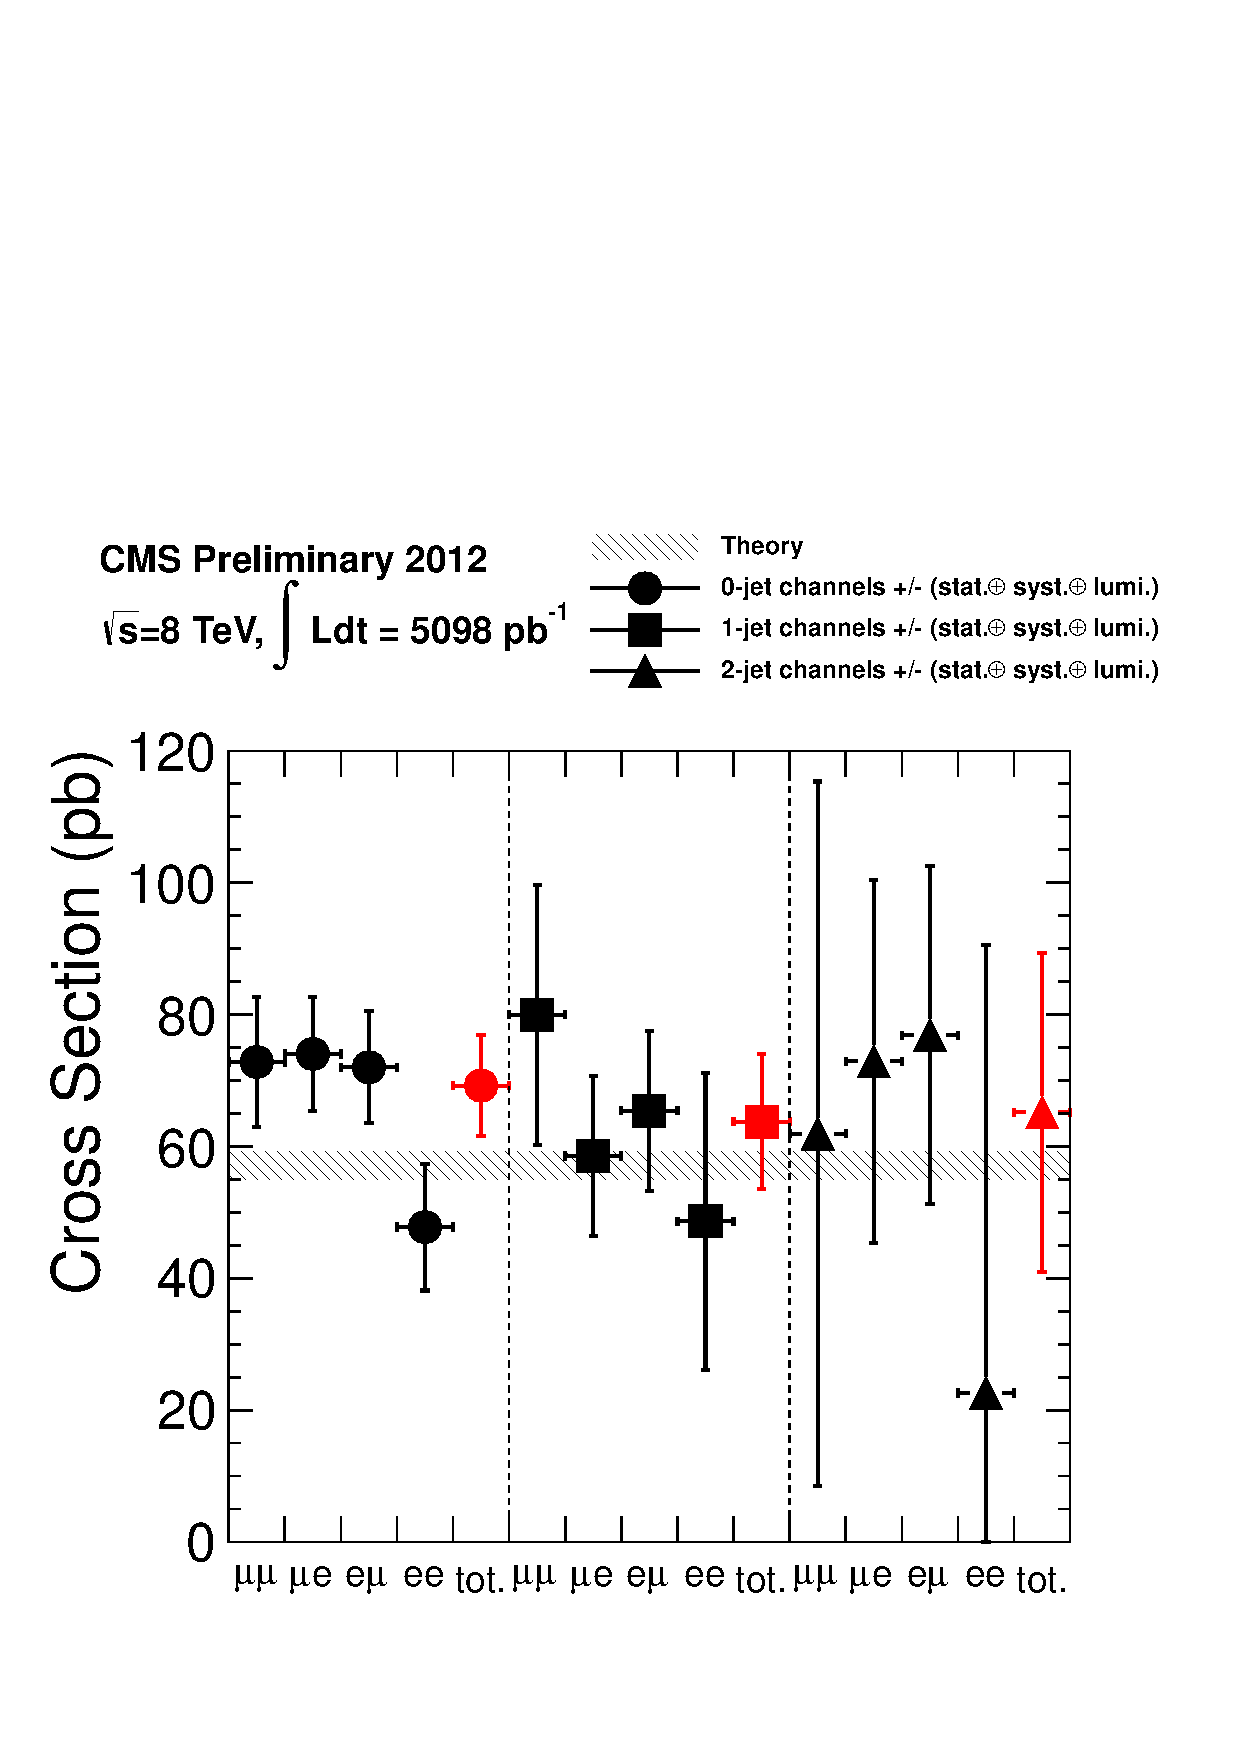
\includegraphics[width=.8\textwidth]{figures/ww_analysis20_0_summary.pdf}
\caption{Summary of all channels. Total uncertainty is shown.}
\label{fig:xs_summary_figure}
\end{figure}




